\documentclass{article}\usepackage[]{graphicx}\usepackage[]{color}
%% maxwidth is the original width if it is less than linewidth
%% otherwise use linewidth (to make sure the graphics do not exceed the margin)
\makeatletter
\def\maxwidth{ %
  \ifdim\Gin@nat@width>\linewidth
    \linewidth
  \else
    \Gin@nat@width
  \fi
}
\makeatother

\definecolor{fgcolor}{rgb}{0.345, 0.345, 0.345}
\newcommand{\hlnum}[1]{\textcolor[rgb]{0.686,0.059,0.569}{#1}}%
\newcommand{\hlstr}[1]{\textcolor[rgb]{0.192,0.494,0.8}{#1}}%
\newcommand{\hlcom}[1]{\textcolor[rgb]{0.678,0.584,0.686}{\textit{#1}}}%
\newcommand{\hlopt}[1]{\textcolor[rgb]{0,0,0}{#1}}%
\newcommand{\hlstd}[1]{\textcolor[rgb]{0.345,0.345,0.345}{#1}}%
\newcommand{\hlkwa}[1]{\textcolor[rgb]{0.161,0.373,0.58}{\textbf{#1}}}%
\newcommand{\hlkwb}[1]{\textcolor[rgb]{0.69,0.353,0.396}{#1}}%
\newcommand{\hlkwc}[1]{\textcolor[rgb]{0.333,0.667,0.333}{#1}}%
\newcommand{\hlkwd}[1]{\textcolor[rgb]{0.737,0.353,0.396}{\textbf{#1}}}%
\let\hlipl\hlkwb

\usepackage{framed}
\makeatletter
\newenvironment{kframe}{%
 \def\at@end@of@kframe{}%
 \ifinner\ifhmode%
  \def\at@end@of@kframe{\end{minipage}}%
  \begin{minipage}{\columnwidth}%
 \fi\fi%
 \def\FrameCommand##1{\hskip\@totalleftmargin \hskip-\fboxsep
 \colorbox{shadecolor}{##1}\hskip-\fboxsep
     % There is no \\@totalrightmargin, so:
     \hskip-\linewidth \hskip-\@totalleftmargin \hskip\columnwidth}%
 \MakeFramed {\advance\hsize-\width
   \@totalleftmargin\z@ \linewidth\hsize
   \@setminipage}}%
 {\par\unskip\endMakeFramed%
 \at@end@of@kframe}
\makeatother

\definecolor{shadecolor}{rgb}{.97, .97, .97}
\definecolor{messagecolor}{rgb}{0, 0, 0}
\definecolor{warningcolor}{rgb}{1, 0, 1}
\definecolor{errorcolor}{rgb}{1, 0, 0}
\newenvironment{knitrout}{}{} % an empty environment to be redefined in TeX

\usepackage{alltt}[12pt]
\usepackage{Sweave}
\usepackage{float}
\usepackage{graphicx}
\usepackage{tabularx}
\usepackage{siunitx}
\usepackage{geometry}
\usepackage{pdflscape}
\usepackage{mdframed}
\usepackage[numbers]{natbib}
\bibliographystyle{..//refs/styles/nature.bst}
\usepackage[small]{caption}
\setlength{\captionmargin}{30pt}
\setlength{\abovecaptionskip}{0pt}
\setlength{\belowcaptionskip}{10pt}
\topmargin -1.5cm        
\oddsidemargin -0.04cm   
\evensidemargin -0.04cm
\textwidth 16.59cm
\textheight 21.94cm 
%\pagestyle{empty} %comment if want page numbers
\parskip 7.2pt
\renewcommand{\baselinestretch}{2}
\parindent 0pt
\usepackage{lineno}
\linenumbers

\newmdenv[
  topline=true,
  bottomline=true,
  skipabove=\topsep,
  skipbelow=\topsep
]{siderules}

%% R Script


\IfFileExists{upquote.sty}{\usepackage{upquote}}{}
\begin{document}
\noindent \textbf{\Large{Rethinking False Spring Risk}}

\section* {How Species Phenological Cues Shape Vegetative Risk}
Predictions of false spring critically depend on understanding what controls the duration of vegetative risk across species. For temperate species, the three major cues (winter chilling temperatures, spring warm temperatures and photoperiod) that control budburst \citep%[e.g., low winter temperatures, warm spring temperatures, and increasing photoperiods]
{Chuine2010} probably play a dominant role. Most phenological studies currently focus on one phenophase (i.e. budburst or leafout) but, in order to examine false spring risk, it is important to examine the effects of the three phenological cues and their interactions on the duration of vegetative risk (i.e. researchers must collect data on both budburst and leafout timing).  

Such cues may provide a starting point for predicting how climate change will alter the duration of vegetative risk. Robust predictions will require more information, especially the emissions scenario realized over coming decades \citep{IPCC2014}, but some outcomes with warming are more expected than others. For example, higher temperatures are generally expected to increase forcing and decrease chilling in many locations, as well as to trigger budburst at times of the year when daylength is shorter. Using data from a recent study that manipulated all three cues and measured budburst and leafout \citep{Flynn2018} shows that any one of these effects alone can have a large impact on the duration of vegetative risk (Figure \ref{fig:dan}): more forcing shortens it substantially (8-15 days), while shorter photoperiods and less chilling increase it to a lesser extent (3-9 days). Together, however, the expected shifts generally shorten the duration of vegetative risk by 4-113 days, both due to the large effect of forcing and the interactive effects of multiple cues. How shortened the risk period is, however varies strongly by species and highlights how climate change may speed some species through this high risk period, but not others. These findings thus show that predictions will require accurate forecasts of the magnitude and direction of how forcing, daylength and chilling will change in the future, as well as how those cues vary across species. 

Considering the interaction of cues and climate change further complicates understanding species future vulnerabilities to false spring events. Most species are expected to begin leafout earlier in the season with warming spring temperatures but some species may have the opposite response due to less winter chilling or decreased photoperiod cues \citep{Cleland2006, Fu2015, Xin2016}. %For example, as climate change progresses, higher spring forcing temperatures may be required for species experiencing insufficient winter chilling (due to warmer winter temperatures), especially at lower latitudes \citep{McCreary1990, Morin2009, Fu2012, Polgar2014, Chuine2010}. 
Individuals that initiate budburst earlier in the spring may attempt to limit freezing risk by decreasing the duration of vegetative risk in order to minimize the exposure of less frost tolerant phenophases \citep{Augspurger2009}. But with a changing climate and thus shifts in phenological cues, this relationship may change \citep{Dolezal2016}. Further studies are essential to understand the interplay between chilling, forcing, and photoperiod cues and the duration of vegetative risk, especially for species occupying ecological niches more susceptible to false spring events. 

\bibliography{..//refs/SpringFreeze.bib}

\begin{figure} [H] 
 \begin{center}
 \textbf{How Major Cues of Spring Phenology Alter Vegetative Risk}\par\medskip
 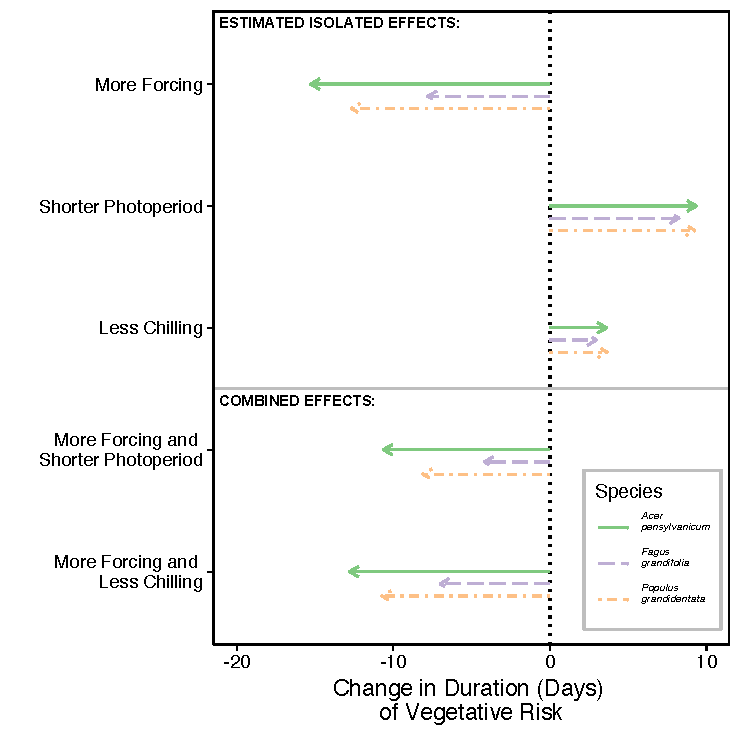
\includegraphics[width=12cm, height=12cm]{..//figure/Exp_plotTPS.pdf} 
 \caption{We examine the effects of phenological cues on the duration of vegatitive risk across three species: \textit{Acer pensylvanicum}, \textit{Fagus grandifolia}, and \textit{Populus grandidentata}. `More Forcing' is a 5$^{\circ}$C increase in forcing temperatures, `Shorter Photoperiod' is a 4 hour decrease in photoperiod and `Less Chilling' is a 30 day decrease in chilling. Along with the estimated isolated effects, we the show the combined predicted shifts in phenological cues with climate change (i.e. more forcing with shorter photoperiod and more forcing with less chilling) and the subsequent shifts in duration of vegetative risk across species. To calculate the interation, we added the two estimated isolated effects to the interaction effect for each species.   }\label{fig:dan} 
 \end{center}
 \end{figure}

\end{document}
